\def\DoNotLoadEpstopdf{}
\documentclass[tikz,border=4pt]{standalone}
% Shared style for the technical appendix figures (2026-10-26).
% Builds on the proposal's figstyle.tex (same fonts, colors, and box styles) and adds
% one encoding for development status, used the same way in every appendix figure.
%   built and tested   solid border (the proposal's normal box styles)
%   built, no test     solid border, and the box text says "no test"
%   specified          dashed border            -> add the key  spec
%   planned            dotted grey border        -> use the style planned
%   no code (by hand)  dotted arrow              -> add the key  byhand
%   outside the artifact  solid grey border      -> use the style outside
% Shared style for proposal figures (2026-10-22 visuals pass).
% Sized to print at 6.5 in (16.5 cm) wide; body text 9 pt sans, nothing below 8 pt.
\usepackage[T1]{fontenc}
\usepackage[scaled=0.95]{helvet}
\renewcommand{\familydefault}{\sfdefault}
\usepackage{xcolor}
\usetikzlibrary{arrows.meta,positioning,calc,patterns.meta}
\definecolor{cink}{HTML}{16191F}
\definecolor{cmuted}{HTML}{4B5563}
\definecolor{cslate}{HTML}{2F4858}
\definecolor{cslatefill}{HTML}{E9EFF3}
\definecolor{cbrass}{HTML}{7A5C12}
\definecolor{cbrassfill}{HTML}{F5EFDE}
\definecolor{cred}{HTML}{8C2F39}
\definecolor{credfill}{HTML}{F8E9EA}
\definecolor{cgreen}{HTML}{235C53}
\definecolor{cgreenfill}{HTML}{E3F0EC}
\definecolor{caudit}{HTML}{5B3A8E}
\definecolor{cauditfill}{HTML}{EFE9F6}
\definecolor{cghost}{HTML}{6B7280}
\definecolor{cghostfill}{HTML}{F3F4F6}
\tikzset{
  >={Triangle[length=5pt,width=4.5pt]},
  box/.style={draw, rounded corners=1.5pt, line width=0.8pt, align=center, inner sep=4pt, font=\fontsize{9}{11}\selectfont},
  sub/.style={font=\fontsize{8}{9.6}\selectfont, text=cmuted},
  ai/.style={box, draw=cbrass, fill=cbrassfill, text=cbrass},
  ver/.style={box, draw=cred, fill=credfill, text=cred},
  pipe/.style={box, draw=cslate, fill=cslatefill, text=cslate},
  prod/.style={box, draw=cslate, fill=cslate, text=white},
  person/.style={box, draw=cink, fill=white, text=cink},
  ghost/.style={box, draw=cghost, fill=cghostfill, text=cghost, dash pattern=on 3pt off 2pt},
  flow/.style={->, line width=0.8pt},
}

\renewcommand{\ttdefault}{lmtt}% vector typewriter font (same design as the default, not a bitmap)
\tikzset{
  spec/.style={dash pattern=on 3pt off 2pt},
  planned/.style={box, draw=cghost, fill=cghostfill, text=cghost, dash pattern=on 0.9pt off 1.6pt},
  outside/.style={box, draw=cghost, fill=white, text=cghost},
  byhand/.style={dash pattern=on 0.9pt off 1.6pt},
  prog/.style={font=\fontsize{8}{9.6}\selectfont\ttfamily},
  legendbox/.style={draw, rounded corners=1pt, line width=0.8pt, minimum width=0.55cm, minimum height=0.32cm, inner sep=0pt},
  legendtext/.style={font=\fontsize{8}{9.6}\selectfont, text=cink, anchor=west, inner sep=1pt},
}
% \statuslegend{x}{y} draws the four-item status legend with its left edge at (x,y).
\newcommand{\statuslegend}[2]{%
  \begin{scope}[shift={(#1,#2)}]
    \node[legendbox, draw=cink, fill=white] (lg1) at (0.275,0) {};
    \node[legendtext] at (0.65,0) {Built and tested};
    \node[legendbox, draw=cink, fill=white, spec] (lg2) at (3.35,0) {};
    \node[legendtext] at (3.725,0) {Specified};
    \node[legendbox, draw=cghost, fill=cghostfill, dash pattern=on 0.9pt off 1.6pt] (lg3) at (5.75,0) {};
    \node[legendtext] at (6.125,0) {Planned};
    \node[legendbox, draw=cghost, fill=white] (lg4) at (7.85,0) {};
    \node[legendtext] at (8.225,0) {Outside the research artifact};
  \end{scope}}

% Figure A7 of the 10/31 appendix: the steps of the verification procedures, in run order.
% Step ids, kinds, and order from verification_procedures/graphs/*.yaml (vg.py topo_order):
% prose.yaml 0.3, citations.yaml 0.2, data.yaml 0.2, build.yaml 0.1, and the three data
% phase reports (data_collection.yaml, data_cleaning.yaml, data_analysis.yaml 0.1), which
% share every step but the first and are drawn once.
\begin{document}
\hyphenpenalty=10000
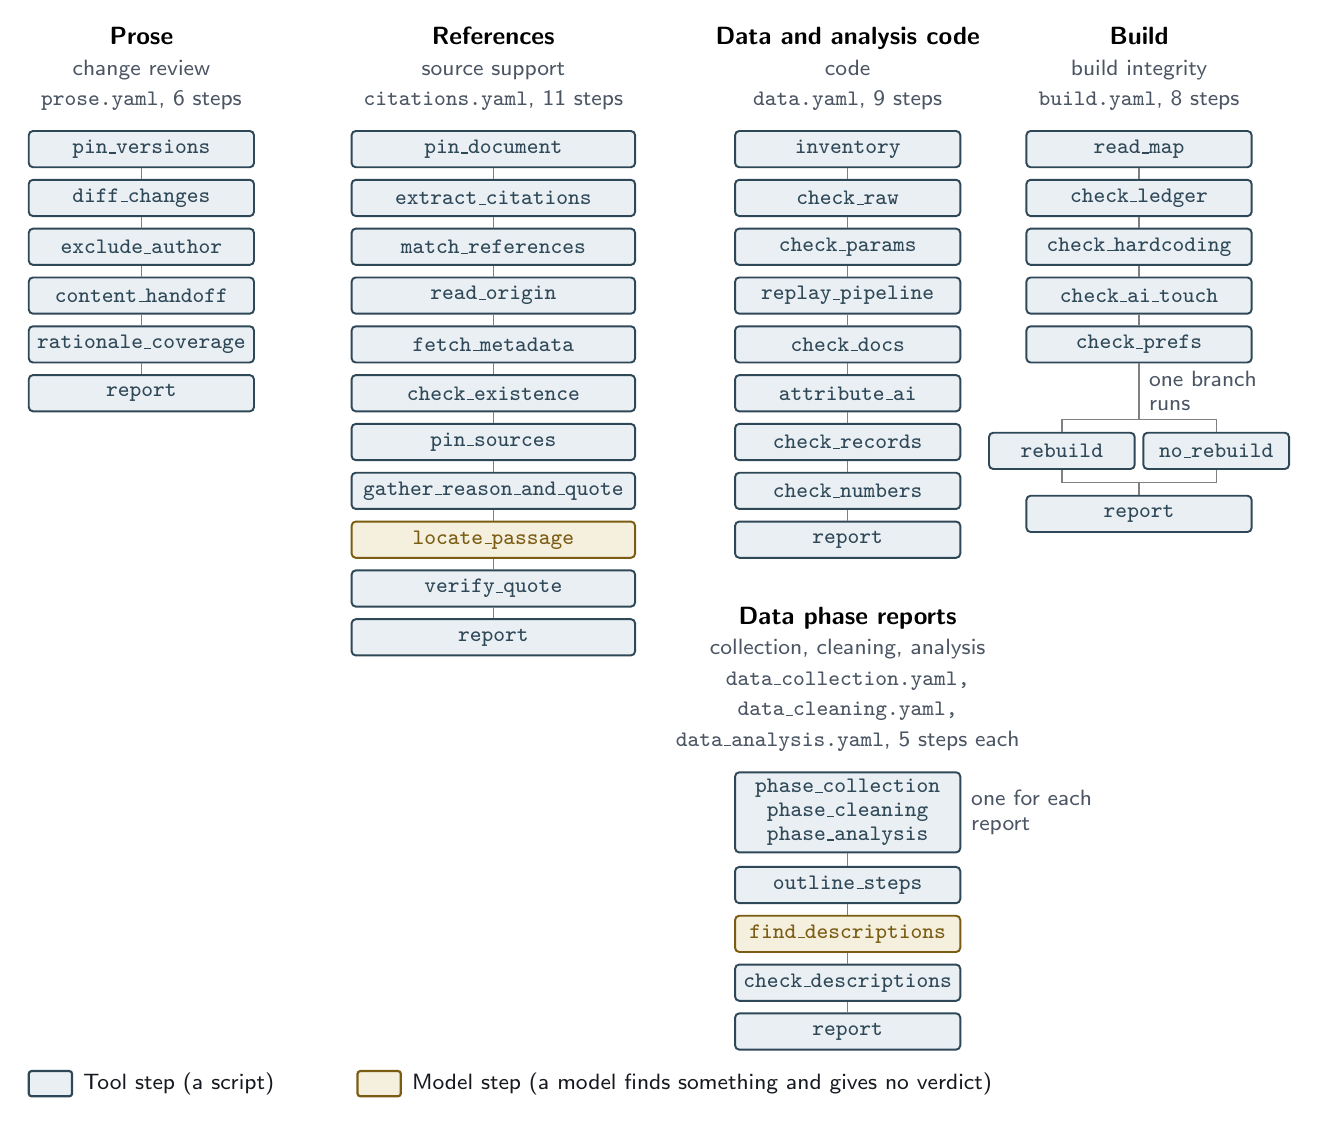
\begin{tikzpicture}
\def\pitch{0.62}
\tikzset{
  stepbox/.style={minimum height=0.46cm, inner sep=1.5pt, line width=0.7pt, rounded corners=1.5pt, prog},
  tool/.style={pipe, stepbox},
  judg/.style={ai, stepbox},
  link/.style={line width=0.5pt, cink!55},
  head/.style={align=center, anchor=south, inner sep=0pt},
  note/.style={font=\fontsize{8}{9}\selectfont, text=cmuted, align=left, anchor=west, inner sep=0pt},
}
\newcommand{\hd}[4]{{\fontsize{9}{11}\selectfont\bfseries #1}\\[-1pt]{\fontsize{8}{9.6}\selectfont\color{cmuted}#2}\\[-1pt]{\fontsize{8}{9.6}\selectfont\color{cmuted}{\ttfamily #3}, #4 steps}}
% column centers and box widths
\def\xP{1.43}  \def\wP{2.86}
\def\xR{5.90}  \def\wR{3.60}
\def\xD{10.40} \def\wD{2.86}
\def\xB{14.10} \def\wB{2.86}
\def\htop{0.48}
% ---------------- headers ----------------
\node[head] at (\xP,\htop) {\hd{Prose}{change review}{prose.yaml}{6}};
\node[head] at (\xR,\htop) {\hd{References}{source support}{citations.yaml}{11}};
\node[head] at (\xD,\htop) {\hd{Data and analysis code}{code}{data.yaml}{9}};
\node[head] at (\xB,\htop) {\hd{Build}{build integrity}{build.yaml}{8}};
% ---------------- prose ----------------
\foreach [count=\i] \s/\k in {pin\_versions/tool, diff\_changes/tool, exclude\_author/tool, content\_handoff/tool, rationale\_coverage/tool, report/tool} {
  \node[\k, minimum width=\wP cm] (p\i) at (\xP,{-(\i-1)*\pitch}) {\s};
}
\foreach \i [evaluate=\i as \j using int(\i+1)] in {1,...,5} {\draw[link] (p\i.south) -- (p\j.north);}
% ---------------- references ----------------
\foreach [count=\i] \s/\k in {pin\_document/tool, extract\_citations/tool, match\_references/tool, read\_origin/tool, fetch\_metadata/tool, check\_existence/tool, pin\_sources/tool, gather\_reason\_and\_quote/tool, locate\_passage/judg, verify\_quote/tool, report/tool} {
  \node[\k, minimum width=\wR cm] (r\i) at (\xR,{-(\i-1)*\pitch}) {\s};
}
\foreach \i [evaluate=\i as \j using int(\i+1)] in {1,...,10} {\draw[link] (r\i.south) -- (r\j.north);}
% ---------------- data ----------------
\foreach [count=\i] \s/\k in {inventory/tool, check\_raw/tool, check\_params/tool, replay\_pipeline/tool, check\_docs/tool, attribute\_ai/tool, check\_records/tool, check\_numbers/tool, report/tool} {
  \node[\k, minimum width=\wD cm] (d\i) at (\xD,{-(\i-1)*\pitch}) {\s};
}
\foreach \i [evaluate=\i as \j using int(\i+1)] in {1,...,8} {\draw[link] (d\i.south) -- (d\j.north);}
% ---------------- data phase reports (under the data column) ----------------
% The three graphs differ only in their first step, which names the phase.
\path let \p1=(d9.south) in \pgfextra{\pgfmathsetmacro{\yq}{\y1/28.4527-2.45}\xdef\yq{\yq}};
\node[head] at (\xD,\yq) {{\fontsize{9}{11}\selectfont\bfseries Data phase reports}\\[-1pt]{\fontsize{8}{9.6}\selectfont\color{cmuted}collection, cleaning, analysis}\\[-1pt]{\fontsize{8}{9.6}\selectfont\color{cmuted}\ttfamily data\_collection.yaml,}\\[-1pt]{\fontsize{8}{9.6}\selectfont\color{cmuted}\ttfamily data\_cleaning.yaml,}\\[-1pt]{\fontsize{8}{9.6}\selectfont\color{cmuted}{\ttfamily data\_analysis.yaml}, 5 steps each}};
\node[tool, minimum width=\wD cm, anchor=north, align=center, inner sep=2.5pt] (q1) at (\xD,\yq-0.25) {phase\_collection\\[-1pt]phase\_cleaning\\[-1pt]phase\_analysis};
\node[note] at ($(q1.east)+(0.12,0)$) {one for each\\report};
\foreach [count=\i from 2] \s/\k in {outline\_steps/tool, find\_descriptions/judg, check\_descriptions/tool, report/tool} {
  \node[\k, minimum width=\wD cm, anchor=north] (q\i) at ($(q1.south)+(0,{-0.16-(\i-2)*\pitch})$) {\s};
}
\foreach \i [evaluate=\i as \j using int(\i+1)] in {1,...,4} {\draw[link] (q\i.south) -- (q\j.north);}
% ---------------- build ----------------
\foreach [count=\i] \s/\k in {read\_map/tool, check\_ledger/tool, check\_hardcoding/tool, check\_ai\_touch/tool, check\_prefs/tool} {
  \node[\k, minimum width=\wB cm] (b\i) at (\xB,{-(\i-1)*\pitch}) {\s};
}
\foreach \i [evaluate=\i as \j using int(\i+1)] in {1,...,4} {\draw[link] (b\i.south) -- (b\j.north);}
\pgfmathsetmacro{\bfork}{-4*\pitch-0.23-0.72}
\pgfmathsetmacro{\bL}{\xB-0.98}
\pgfmathsetmacro{\bRt}{\xB+0.98}
\node[tool, minimum width=1.85cm, anchor=north] (bA) at (\bL,\bfork-0.16) {rebuild};
\node[tool, minimum width=1.85cm, anchor=north] (bB) at (\bRt,\bfork-0.16) {no\_rebuild};
\draw[link] (b5.south) -- (\xB,\bfork);
\draw[link] (\bL,\bfork) -- (\bRt,\bfork);
\draw[link] (\bL,\bfork) -- (bA.north);
\draw[link] (\bRt,\bfork) -- (bB.north);
\node[note] at (\xB+0.12,{-4*\pitch-0.23-0.36}) {one branch\\runs};
\pgfmathsetmacro{\bmerge}{\bfork-0.16-0.46-0.18}
\draw[link] (bA.south) -- (\bL,\bmerge) -- (\bRt,\bmerge) -- (bB.south);
\node[tool, minimum width=\wB cm, anchor=north] (b8) at (\xB,\bmerge-0.16) {report};
\draw[link] (\xB,\bmerge) -- (b8.north);
% ---------------- key ----------------
\path let \p1=(q5.south) in \pgfextra{\pgfmathsetmacro{\ky}{\y1/28.4527-0.42}\xdef\ky{\ky}};
\node[legendbox, draw=cslate, fill=cslatefill] at (0.275,\ky) {};
\node[legendtext] at (0.65,\ky) {Tool step (a script)};
\node[legendbox, draw=cbrass, fill=cbrassfill] at (4.45,\ky) {};
\node[legendtext] at (4.825,\ky) {Model step (a model finds something and gives no verdict)};
\end{tikzpicture}
\end{document}
